
%\section{Multi-Agent Systems Review}
An essential concept which is repeatedly referred to in this thesis is that of an agent. The term "agent" is an abstract one with no single definition universally accepted in the literature. Most definitions agree reasonably closely with the one provided in AI: A Modern Approach by Russell and Norvig: An agent is "anything that can be viewed as perceiving its environment through sensors and acting upon that environment through actuators."\cite{AIAMA}. \mynote{Figures won't render properly, not sure why exactly}
Figure\ref{fig:agent_env_interaction} helps to illustrate this concept: \begin{figure}
    \centering
    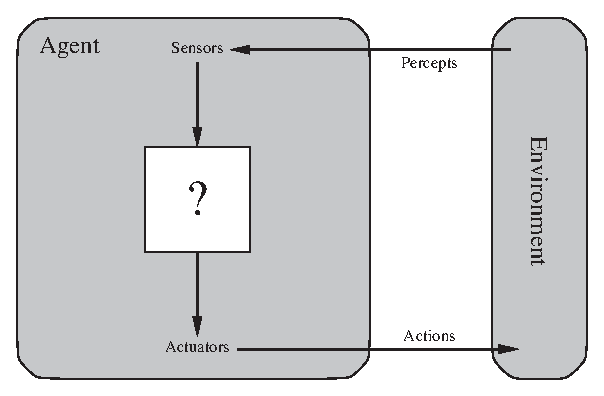
\includegraphics{Chapters/BackgroundKnowledgeAndRelatedWork/Figs/Vector/agent-environment.eps}
    \caption{Agent Environment Interacation}
    \label{fig:agent_env_interaction}
\end{figure}

Agents are usually assumed to act in an environment, which comprises of everything external to the agent, which provides percepts and may change through actuation.

An agent is usually intuitively interpreted as an entity that acts on the behalf of a person on people in order to accomplish some high-level task.\par


To define a Multi-Agent System, it is instructive to first define the field from which it stems, Distributed Artificial Intelligence (DAI). A definition from Peter Stone states "DAI is concerned with systems that consist of multiple independent entities that interact in a domain."\cite{Stone2000MultiagentPerspective}
